\chapter{Validação do Sistema (Resultados e Discussão)}

Este capítulo apresenta os resultados da validação do sistema Test-Manager junto aos usuários que atuaram nos papéis de Coordenador, Tester e Desenvolvedor em projetos de software do IFES Campus Alegre. O delineamento metodológico geral da avaliação foi descrito no Capítulo 3; nesta seção detalham-se o instrumento ramificado por perfil, o protocolo de coleta, a tabulação estatística das respostas e a discussão dos achados em relação aos objetivos do trabalho.

\section{Instrumentos de Avaliação}

A validação foi estruturada em dois níveis complementares: (i) verificação técnica funcional por lista de checagem (\textit{checklist}) dos fluxos operacionais e restrições de acesso por perfil; e (ii) avaliação perceptiva dos usuários por meio de questionário estruturado fundamentado no Modelo de Aceitação de Tecnologia (\textit{Technology Acceptance Model} --- TAM) \cite{davis1989, venkatesh2000} e em preceitos de engenharia de usabilidade \cite{nielsen1994}.

\subsection{Verificação Técnica}

Antes da aplicação do questionário, foram exercitados manualmente os fluxos principais do sistema em ambiente conteinerizado: cadastro de projetos e alocação de equipes pelo Coordenador, importação de roteiros de teste em lote via arquivo \texttt{.csv}, atribuição e avaliação de versões pelo Tester, exigência de cadastro de defeito com upload de captura de tela (\textit{print}) no fluxo de reprovação, atualização de status de correção pelo Desenvolvedor e geração de logs de auditoria e relatórios em PDF. Confirmou-se que as regras de negócio modeladas no Capítulo 4 refletem-se integralmente no comportamento da aplicação, sem falhas de permissão entre perfis.

\subsection{Questionário de Avaliação (Modelo TAM)}

O questionário foi elaborado na plataforma Google Forms e organizado em blocos lógicos. O primeiro bloco coletou o perfil de acesso principal utilizado pelo participante e apresentou oito afirmações gerais (Q1 a Q8), respondidas por todos os integrantes, abrangendo os construtos de \textbf{Facilidade de Uso Percebida} (Q1 a Q3), \textbf{Utilidade Percebida} (Q4 a Q6) e \textbf{Intenção Comportamental de Uso} (Q7 e Q8).

Na sequência, o formulário utilizou ramificação condicional para avaliar as funcionalidades exclusivas de cada ator: o perfil \textbf{Coordenador} respondeu aos itens Q9 a Q11; o perfil \textbf{Tester} avaliou os itens Q12 a Q14; e o perfil \textbf{Desenvolvedor} respondeu aos itens Q15 a Q17. Todas as afirmações fechadas foram mensuradas em escala Likert de cinco pontos, variando de 1 (\textit{Discordo Totalmente}) a 5 (\textit{Concordo Totalmente}). Ao final, duas questões abertas (Q18 e Q19) coletaram percepções sobre dificuldades encontradas e sugestões de evolução futura. O Quadro \ref{quad:itens_questionario} detalha a estrutura completa do instrumento aplicado.

\begin{quadro}[!htb]
\centering
\caption{Itens do formulário de avaliação do sistema Test-Manager.}
\label{quad:itens_questionario}
\footnotesize
\begin{tabularx}{\textwidth}{|p{1.1cm}|p{3.3cm}|X|}
\hline
\textbf{Cód.} & \textbf{Dimensão / Escopo} & \textbf{Afirmação / Questão} \\ \hline
Perfil & Identificação & Qual é o seu perfil de acesso principal no Test-Manager? (Coordenador, Tester ou Desenvolvedor). \\ \hline
Q1 & Facilidade de Uso (Geral) & Aprender a utilizar o Test-Manager foi um processo fácil e rápido para mim. \\ \hline
Q2 & Facilidade de Uso (Geral) & A interface do sistema é clara, intuitiva e fácil de navegar. \\ \hline
Q3 & Facilidade de Uso (Geral) & É fácil encontrar as informações ou funcionalidades que preciso dentro do sistema. \\ \hline
Q4 & Utilidade Percebida (Geral) & O uso do Test-Manager torna o processo mais rápido em comparação ao método anterior (planilhas/Google Docs). \\ \hline
Q5 & Utilidade Percebida (Geral) & O sistema ajuda a manter o histórico de testes e falhas de forma mais segura e rastreável. \\ \hline
Q6 & Utilidade Percebida (Geral) & Em geral, acredito que o Test-Manager melhora a minha produtividade no projeto. \\ \hline
Q7 & Intenção de Uso (Geral) & Pretendo continuar utilizando o Test-Manager nas atividades de QA dos próximos projetos. \\ \hline
Q8 & Intenção de Uso (Geral) & Eu recomendaria este sistema para outras equipes de desenvolvimento do IFES. \\ \hline
Q9 & Específico: Coordenador & O processo de criar projetos e vincular Desenvolvedores e Testers é simples e direto. \\ \hline
Q10 & Específico: Coordenador & O sistema me oferece uma boa visão geral sobre o andamento da qualidade dos projetos. \\ \hline
Q11 & Específico: Coordenador & A importação em lote de casos de teste via arquivo CSV agiliza a alimentação inicial do sistema. \\ \hline
Q12 & Específico: Tester & A tela de listagem de Casos de Teste permite entender rapidamente os passos e o resultado esperado. \\ \hline
Q13 & Específico: Tester & O processo de aprovar ou reprovar uma versão de teste é ágil e requer poucos cliques. \\ \hline
Q14 & Específico: Tester & A obrigatoriedade de cadastrar um defeito (\textit{bug}) ao reprovar um teste ajuda a garantir a documentação da falha. \\ \hline
Q15 & Específico: Desenvolvedor & É fácil visualizar e filtrar os defeitos (\textit{bugs}) que foram atribuídos ao meu projeto. \\ \hline
Q16 & Específico: Desenvolvedor & As informações fornecidas na tela de Detalhes do Defeito são claras e suficientes para eu corrigir o erro. \\ \hline
Q17 & Específico: Desenvolvedor & Atualizar o ciclo de vida do defeito facilita a comunicação com a equipe sem usar ferramentas externas. \\ \hline
Q18 & Aberta (Dificuldades) & Qual foi a maior dificuldade ou confusão que você encontrou ao utilizar o sistema? \\ \hline
Q19 & Aberta (Sugestões) & Quais funcionalidades você sugere que sejam adicionadas, alteradas ou removidas no futuro? \\ \hline
\end{tabularx}
\fonte{Elaborado pelo autor (2026).}
\end{quadro}

\section{Procedimento de Coleta}

O procedimento adotado na condução da avaliação empírica seguiu cinco etapas:
\begin{enumerate}
    \item Disponibilização do Test-Manager aos participantes atuantes em projetos de software no IFES Campus Alegre, com orientação inicial conforme o perfil de acesso;
    \item Período de uso orientado do sistema contemplando os fluxos de criação de projetos, importação e cadastro de casos de teste, execução e avaliação de versões, relato obrigatório de defeitos na reprovação e resolução de \textit{bugs};
    \item Divulgação do link do formulário eletrônico aos usuários que operaram a plataforma;
    \item Coleta anônima das respostas por meio do Google Forms entre outubro e novembro de 2026;
    \item Tabulação quantitativa das respostas em escala Likert (médias aritméticas e desvios-padrão amostrais) e análise qualitativa das respostas discursivas.
\end{enumerate}

Não houve identificação nominal dos participantes; o perfil declarado serviu exclusivamente para direcionar o bloco de questões específicas e contextualizar a análise dos resultados.

\section{Resultados}

A coleta obteve 5 respostas válidas ($n = 5$) após o uso orientado do Test-Manager. Quanto ao perfil de acesso principal declarado, a amostra contemplou todos os atores modelados no sistema, distribuindo-se em: Coordenador (1), Tester (2) e Desenvolvedor (2).

A Tabela \ref{tab:resultados_likert} consolida o número de respondentes ($n$), as médias e os desvios-padrão (DP) obtidos em cada afirmação na escala de 1 a 5. De forma complementar, a Figura \ref{fig:grafico_pizza_concordancia} apresenta em gráficos de setores (pizza) a proporção percentual das notas atribuídas no bloco geral (Q1 a Q8) e nos módulos específicos por perfil (Q9 a Q17), enquanto a Figura \ref{fig:grafico_pizza_dimensoes_tam} detalha a distribuição percentual de concordância estratificada pelas três dimensões do Modelo TAM.

\begin{table}[H]
\centering
\caption{Resultados do questionário de avaliação do Test-Manager (Escala Likert 1--5).}
\label{tab:resultados_likert}
\small
\begin{tabularx}{\textwidth}{|l|X|c|c|c|}
\hline
\textbf{Item} & \textbf{Aspecto Avaliado} & \textbf{$n$} & \textbf{Média} & \textbf{DP} \\ \hline
\multicolumn{5}{|l|}{\textbf{Dimensões Gerais do Modelo TAM (Todos os Perfis)}} \\ \hline
Q1 & Facilidade e rapidez no aprendizado do sistema & 5 & 4,20 & 0,45 \\ \hline
Q2 & Clareza, intuitividade e navegabilidade da interface & 5 & 4,40 & 0,89 \\ \hline
Q3 & Facilidade para localizar informações e funcionalidades & 5 & 4,20 & 0,84 \\ \hline
Q4 & Agilidade do processo frente a planilhas/Google Docs & 5 & 4,40 & 0,89 \\ \hline
Q5 & Segurança e rastreabilidade do histórico de testes e falhas & 5 & 4,80 & 0,45 \\ \hline
Q6 & Melhoria da produtividade nas atividades do projeto & 5 & 4,60 & 0,55 \\ \hline
Q7 & Intenção de uso contínuo nos próximos projetos & 5 & 4,60 & 0,55 \\ \hline
Q8 & Recomendação do sistema para outras equipes do IFES & 5 & 4,20 & 1,30 \\ \hline
\multicolumn{5}{|l|}{\textbf{Módulos Específicos por Perfil de Acesso}} \\ \hline
Q9 & Simplicidade ao criar projetos e vincular equipe (Coordenador) & 1 & 4,00 & - \\ \hline
Q10 & Visão geral sobre o andamento da qualidade (Coordenador) & 1 & 5,00 & - \\ \hline
Q11 & Agilidade na importação em lote via arquivo CSV (Coordenador) & 1 & 5,00 & - \\ \hline
Q12 & Clareza dos passos e resultado esperado na listagem (Tester) & 2 & 4,50 & 0,71 \\ \hline
Q13 & Agilidade ao aprovar ou reprovar versões de teste (Tester) & 2 & 5,00 & 0,00 \\ \hline
Q14 & Documentação garantida pelo defeito obrigatório na reprovação (Tester) & 2 & 5,00 & 0,00 \\ \hline
Q15 & Facilidade ao visualizar e filtrar defeitos atribuídos (Desenvolvedor) & 2 & 4,50 & 0,71 \\ \hline
Q16 & Suficiência das informações nos detalhes do defeito (Desenvolvedor) & 2 & 5,00 & 0,00 \\ \hline
Q17 & Comunicação facilitada pela atualização do ciclo de vida (Desenvolvedor) & 2 & 5,00 & 0,00 \\ \hline
\multicolumn{2}{|l|}{\textbf{Média Geral dos Itens Comuns (Q1--Q8)}} & \textbf{40 obs.} & \textbf{4,43} & \textbf{0,75} \\ \hline
\multicolumn{2}{|l|}{\textbf{Média Geral dos Módulos Específicos (Q9--Q17)}} & \textbf{15 obs.} & \textbf{4,80} & \textbf{0,41} \\ \hline
\multicolumn{2}{|l|}{\textbf{Média Global Consolidada (Q1--Q17)}} & \textbf{55 obs.} & \textbf{4,53} & \textbf{0,69} \\ \hline
\end{tabularx}
\fonte{Elaborado pelo autor (2026), com base na aplicação do questionário.}
\end{table}

\begin{figure}[H]
    \centering
    \caption{Proporção percentual de concordância na Escala Likert: (a) Dimensões Gerais (Q1 a Q8) e (b) Funcionalidades Específicas por Perfil (Q9 a Q17).}
    \label{fig:grafico_pizza_concordancia}
    \vspace{0.2cm}
    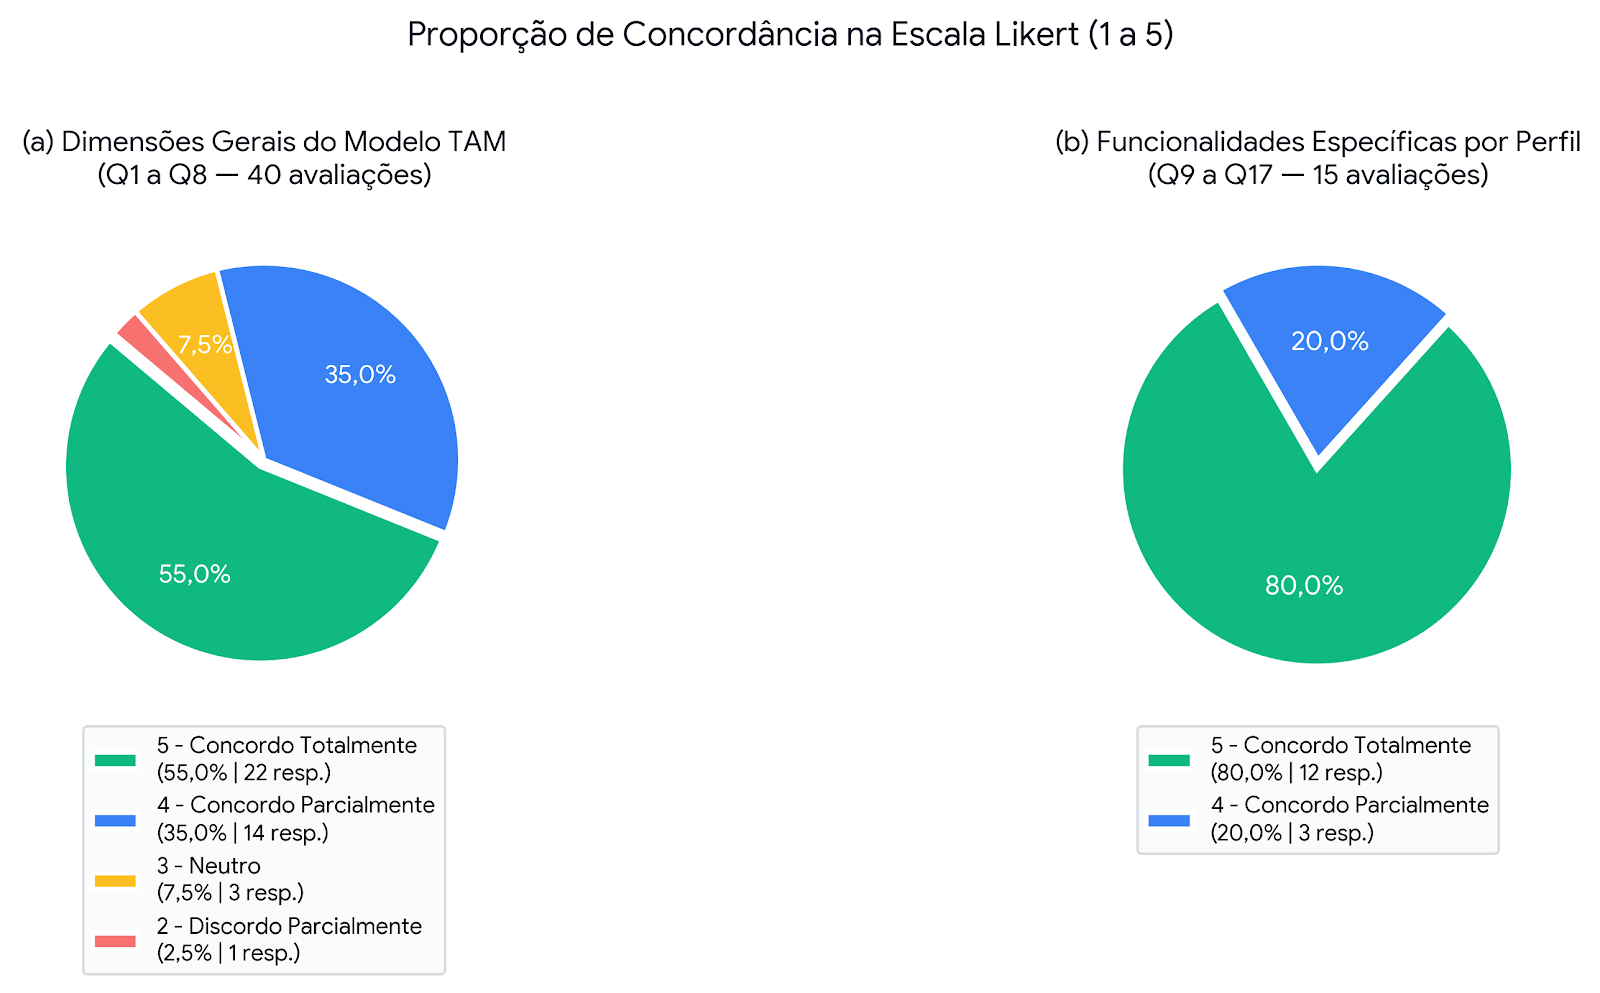
\includegraphics[width=0.95\textwidth, keepaspectratio]{./figuras/grafico_pizza_concordancia.png} \\
    \vspace{0.2cm}
    {\raggedright \small Fonte: Elaborado pelo autor (2026).\par}
\end{figure}

\begin{figure}[H]
    \centering
    \caption{Distribuição percentual das respostas por dimensão do Modelo TAM: (a) Facilidade de Uso, (b) Utilidade Percebida e (c) Intenção de Uso.}
    \label{fig:grafico_pizza_dimensoes_tam}
    \vspace{0.2cm}
    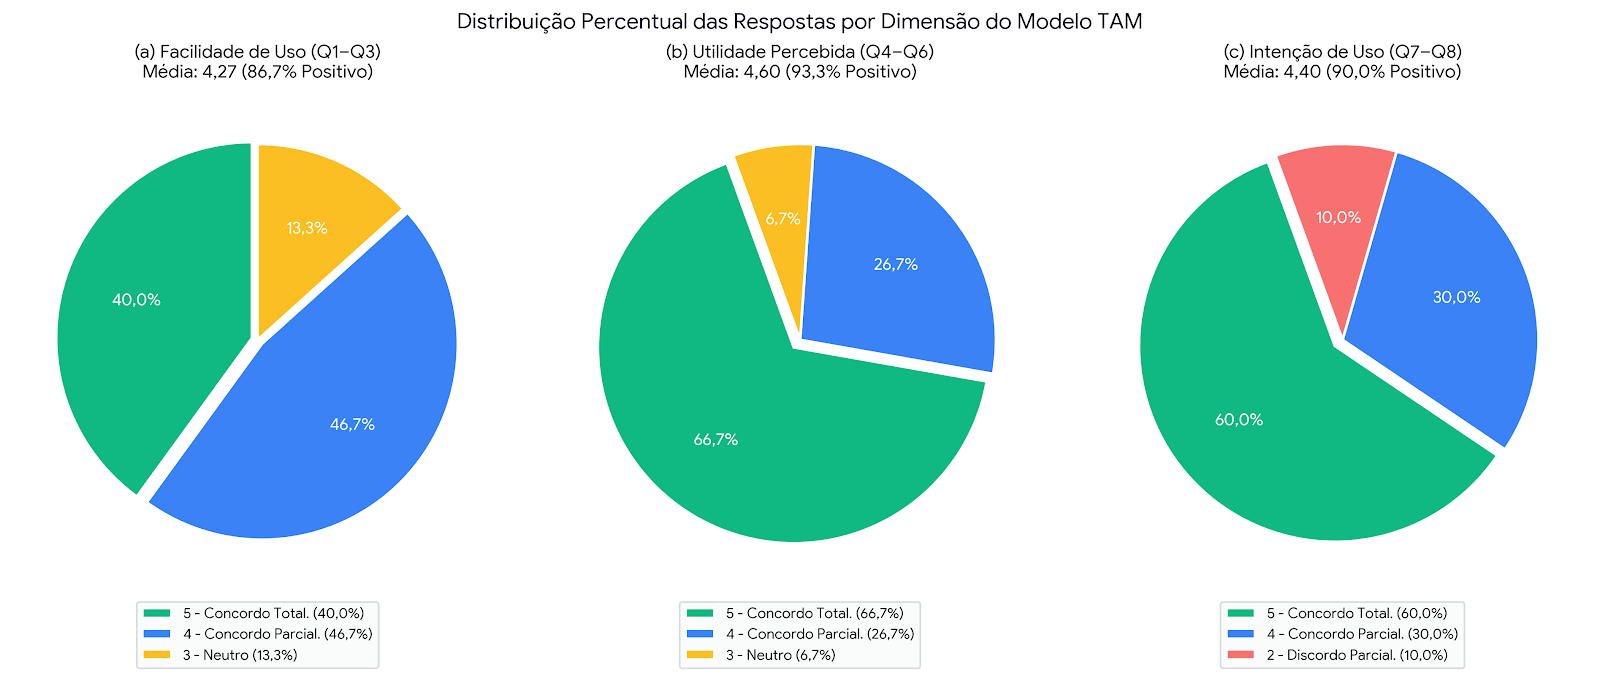
\includegraphics[width=0.98\textwidth, keepaspectratio]{./figuras/grafico_pizza_dimensoes_tam.png} \\
    \vspace{0.2cm}
    {\raggedright \small Fonte: Elaborado pelo autor (2026).\par}
\end{figure}

\subsection{Respostas Abertas: Dificuldades e Sugestões (Q18 e Q19)}

Nas questões discursivas destinadas ao levantamento de dificuldades operacionais (Q18) e sugestões de aprimoramento futuro (Q19), quatro participantes registraram observações sobre dificuldades e três indicaram propostas de evolução:
\begin{itemize}
    \item \textbf{Perfil Coordenador:} Relatou que sua expectativa inicial era de que a plataforma também abrangesse o gerenciamento prévio de requisitos do software, sugerindo para trabalhos futuros a inclusão de um módulo de cadastro de requisitos formalmente atrelado aos casos de teste, além do refinamento contínuo nas nomenclaturas de status de testes e níveis de prioridade de defeitos;
    \item \textbf{Perfil Tester:} Um avaliador apontou como limitação pontual o fato de o formulário de relato de defeito permitir o envio de apenas uma captura de tela (\textit{print}) por registro; o segundo avaliador mencionou dificuldade visual para localizar de imediato os botões de edição e exclusão logo após cadastrar um caso de teste, sugerindo destacá-los na interface de listagem;
    \item \textbf{Perfil Desenvolvedor:} Ambos os respondentes indicaram não ter encontrado nenhuma dificuldade ou confusão ao operar o sistema (``Nenhuma''), e um deles corroborou a sugestão de permitir o anexo de múltiplos arquivos ou imagens no registro de defeitos para enriquecer a evidência do erro.
\end{itemize}

\section{Discussão}

Conforme demonstrado na Tabela \ref{tab:resultados_likert} e ilustrado nos gráficos de setores das Figuras \ref{fig:grafico_pizza_concordancia} e \ref{fig:grafico_pizza_dimensoes_tam}, a avaliação empírica evidenciou ampla aceitação do sistema Test-Manager após o uso prático. Na Figura \ref{fig:grafico_pizza_concordancia}(a), observa-se que, das 40 avaliações individuais realizadas nas questões gerais (Q1 a Q8), expressivos \textbf{90,0\%} concentraram-se na faixa positiva de concordância --- sendo \textbf{55,0\%} (22 respostas) em \textit{Concordo Totalmente} (nota 5) e \textbf{35,0\%} (14 respostas) em \textit{Concordo Parcialmente} (nota 4) ---, frente a apenas 7,5\% (3 respostas) de posicionamento neutro e 2,5\% (1 resposta) de discordância parcial, resultando na média geral comum de 4,43 ($\text{DP} = 0,75$).

Analisando a Figura \ref{fig:grafico_pizza_dimensoes_tam}, que decompõe o resultado geral nas três dimensões teóricas do Modelo TAM \cite{davis1989, venkatesh2000}, verifica-se o predomínio das fatias de aprovação (verde e azul) em todos os construtos:
\begin{itemize}
    \item Na \textbf{Utilidade Percebida} (Figura \ref{fig:grafico_pizza_dimensoes_tam}b, referente aos itens Q4 a Q6), o índice de concordância positiva atingiu \textbf{93,3\%}, com dois terços das respostas (\textbf{66,7\%}) na nota máxima (\textit{Concordo Totalmente}) e média agregada de 4,60 ($\text{DP} = 0,63$). O destaque recaiu sobre o item Q5 (manutenção do histórico de testes e falhas de forma segura e rastreável, média 4,80), confirmando que a centralização em banco relacional supera a perda de histórico típica de planilhas e documentos soltos em nuvem \cite{medeiros2022, kokubum2025};
    \item Na \textbf{Facilidade de Uso Percebida} (Figura \ref{fig:grafico_pizza_dimensoes_tam}a, itens Q1 a Q3), \textbf{86,7\%} das respostas situaram-se entre \textit{Concordo Totalmente} (40,0\%) e \textit{Concordo Parcialmente} (46,7\%), com 13,3\% de neutralidade e nenhuma discordância (média de 4,27; $\text{DP} = 0,70$), validando a intuitividade da interface construída com Bootstrap 5;
    \item Na \textbf{Intenção Comportamental de Uso} (Figura \ref{fig:grafico_pizza_dimensoes_tam}c, itens Q7 e Q8), \textbf{90,0\%} das avaliações foram positivas (60,0\% em \textit{Concordo Totalmente} e 30,0\% em \textit{Concordo Parcialmente}, média 4,40). Os 10,0\% correspondentes a uma única resposta \textit{Discordo Parcialmente} (nota 2 em Q8) referem-se à cautela apontada pelo perfil Coordenador na questão aberta (Q18/Q19), que sugeriu incorporar um módulo prévio de Engenharia de Requisitos antes de expandir a recomendação da ferramenta para outras equipes.
\end{itemize}

Por fim, o gráfico da Figura \ref{fig:grafico_pizza_concordancia}(b) evidencia o desempenho superior do sistema na execução das rotinas específicas de cada papel (\textbf{Módulos Específicos por Perfil}, Q9 a Q17): \textbf{100,0\%} das 15 avaliações foram positivas, sendo \textbf{80,0\%} (12 respostas) de aprovação máxima (\textit{Concordo Totalmente}, nota 5) e \textbf{20,0\%} (3 respostas) de concordância parcial (nota 4), elevando a média específica para \textbf{4,80} ($\text{DP} = 0,41$). Seis dos nove indicadores específicos obtiveram nota máxima unânime (5,00): visão geral da qualidade (Q10) e importação em lote via CSV (Q11) no perfil Coordenador; agilidade ao aprovar/reprovar versões (Q13) e obrigatoriedade de abertura de defeito na reprovação (Q14) no perfil Tester; e clareza nos detalhes do defeito (Q16) e facilidade de comunicação pelo ciclo de vida (Q17) no perfil Desenvolvedor.

As sugestões registradas nas questões abertas --- suporte a múltiplos anexos de imagem por defeito, maior destaque visual aos botões de edição/exclusão para o perfil Tester e criação de um módulo de rastreabilidade de requisitos --- oferecem um direcionamento claro para a evolução contínua da plataforma, detalhado no Capítulo 7.